
\begin{sidewaysfigure}[ht!]
\tikzset{edge from parent/.style=
{draw, edge from parent path={(\tikzparentnode.south)
-- +(0,-8pt)
-| (\tikzchildnode)}},
blank/.style={draw=none}}
\begin{tikzpicture}
\matrix
{
\node{\Tree
    [.\textbf{ }  \edge[blank]; 
    [.\textbf{Topic}  \edge[blank];
    [.\textbf{News\ event} \edge[blank]; 
    [.\textbf{Article} ]]]]};
&
\node{\Tree 
 [.All\ news 
    [.Politics 
        [.Parliamentary\ debate\ on\ X  1 2 3 ] 
        [.Local\ election\ result\ in\ X  1 ] 
        ]
    [.Accidents,\ disasters,\ ... 
        [.Accident\ on\ highway\ Y  1 2 3 4 5 6 ] ]
    [.Sports
        [.Club\ A\ defeats\ club\ B 1 2 3 ] ]
        ]}; \\
};        
\end{tikzpicture}
\caption{News events can be covered by one or more articles in one or more outlets, but relate to one specific and identifiable event and are thus much more fine-grained than news topics or news categories. \label{fig:model}}
\end{sidewaysfigure}
